%% This is an example first chapter.  You should put chapter/appendix that you
%% write into a separate file, and add a line \include{yourfilename} to
%% main.tex, where `yourfilename.tex' is the name of the chapter/appendix file.
%% You can process specific files by typing their names in at the 
%% \files=
%% prompt when you run the file main.tex through LaTeX.
\chapter{Introduction}

\section{The Standard Model of Particle Physics}

Physics is the research of relationship between space and time and energy and matter. Physicists enjoy searching for symmetries and consideration laws in nature. They develop elegant mathematical formulations to describe the beauty of the nature and predict or explain the experimental results and observed phenomena. 

There are four known fundamental forces in nature: gravitational force, electromagnetic force, strong force, and weak force. The gravitation force describes the interaction between two massive objects. The electromagnetic force describe the interaction between electrically charged objects. The strong force describes the interaction between nucleons. The weak force describe the radioactive decay of particles. The Standard Model (SM) of Particle Physics is based on theoretical of relativistic quantum field theory with a gauge symmetry of $SU(3) \times SU(2) \times U(1)$ \cite{SMTheory}. It unifies the strong, weak, and electromagnetic into a single theory and describes all particles participating in these interactions. The ingredient of the standard model are lepton, quarks, gauge boson, and Higgs boson shown in Figure~\ref{fig:SMParticle}.

\begin{figure}[hbtp]
\begin{center}
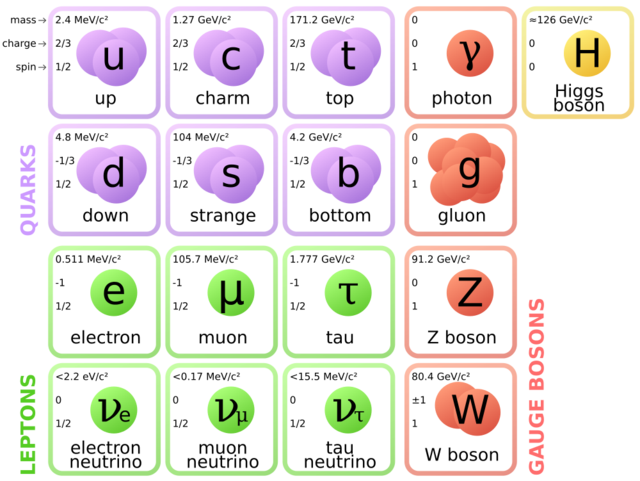
\includegraphics[width=0.50\textwidth]{Figures/Chapter1/SMParticles.png}
\caption{The 17 elementary particles, including leptons, quarks, gauge bosons, and Higgs boson, and their basic properties, such as mass, electric charge, spin, in the Standard Model of Particles Physics are shown above.}
\label{fig:SMParticle}
\end{center}
\end{figure} 


There are 19 parameters in the Standard Model: 6 quark masses, 3 lepton masses, 3 coupling strengths, 4 CKM angles, Higgs mass, vacuum expectation value, and QCD vacuum angle. These parameters are determined from the experiments. Physicists perform calculations based on the Standard Model and predict the cross section of different processes in high energy physics experiments. Since it is proposed in the 1970s, the Standard Model has been tested extensively in countless high-energy physics experiments. Its prediction holds for all of them with very few exceptions. The Standard Model consists of two sectors: the Electroweak theory (EW) and Quantum Chromodynamics (QCD). The Lagrangian of the Standard Model can be written as the sum of EW and QCD: $\mathcal{L_{SM}} = \mathcal{L_{EW}} + \mathcal{L_{QCD}}$ 


\section{Quantum Chromodynamics}

\subsection{QCD Lagrangian}

QCD, a non-abelian gauge theory with $SU(3)$ symmetry, is the theory for the strong interaction between quarks and gluons. The QCD Lagrangian is as follows:


\begin{equation}
\mathcal{L_{QCD}} = \bar \Psi^i i (\slashed{D})_{ij} \Psi^j - m  \bar \Psi^i \Psi_i - \frac{1}{16\pi^2} G^{\mu\nu}_{a}G_{\mu\nu}^{a}
\end{equation}

Where 

\begin{equation}
\slashed{D} = \gamma^\mu \partial_\mu - i g_s \frac{\lambda}{2}  \gamma^\mu A_\mu
\end{equation}

\begin{equation}
G^{\mu\nu}_{a} = \partial^\mu A^\nu_{a} - \partial_{\nu} A^\mu_{a} + g_s f_{abc} A^\mu_b A^\nu_c 
\end{equation}

Here, $\lambda$ are the Gell-Mann Matrices. $f_{abc}$ is the structure of constant of $SU(3)$. $A^\mu$ is the eight gluon field. $g_s$ is the strong coupling constant. The color indices $i$ and $j$ run from 1 to 3, which stands for 3 colors: red, blue, and green. The gluon field indices $a$, $b$, and $c$ run from 1 to 8, standing for the 8 gluon state (Gluon octet as the combination of 3 color and 3 anticolor: $3 \times \bar 3 = 1 \oplus 8$) living in the adjoint representation of $SU(3)$ of color.  



\subsection{Asymptotic Freedom}

The running of the strong coupling constant $\alpha_s = \frac{g_s^2}{4\pi}$ according to the 1-loop calculations in the renomalization theory \cite{QCDRunning} is shown as follows

\begin{equation}
\alpha_{s} (Q^2) = \frac{12\pi}{(11 N_{c} - 2 N_{f}) \ln(\frac{Q^2}{\Lambda_{QCD}^2})}
\end{equation}

We can see that as the energy scale increases, the coupling strength of the strong interaction decreases. This is in contrast to QED where the electromagnetic coupling strength increases as the energy scale increases. In the ultra-violate limit $Q^2 \rightarrow \infty$ and $\alpha_{s} \rightarrow 0$, quarks and gluons behave like free particles. This feature in QCD is call Asymptotic Freedom \cite{QCDAsym}. Meanwhile, in the infrared limit, the strong coupling constant increases. Near the $\Lambda_{QCD} \simeq$100 MeV, the coupling is greater than 1, where the perturbative expansion of QCD breaks down. Experimentally, physicists measure the strong coupling constant at different energy scales from different experiments at different colliders. Figure~\ref{QCDCoupling} \cite{AlphaTheoEx} show the running of strong coupling constant in experiment and comparison with the theoretical calculations 

\begin{figure}[hbtp]
\begin{center}
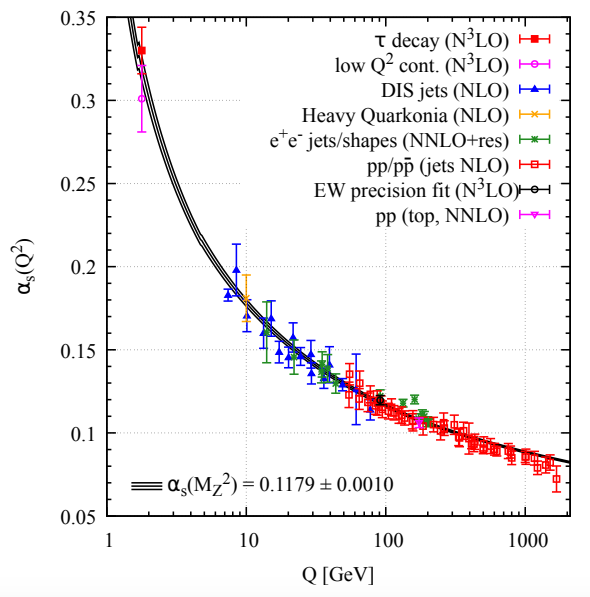
\includegraphics[width=0.50\textwidth]{Figures/Chapter1/QCDCoupling.png}
\caption{The running of the strong coupling constant $\alpha_s$ in different experiments at different energy scale $Q$ and the comparison with QCD calculations are shown above.}
\label{QCDCoupling}
\end{center}
\end{figure} 

An excellent agreement between the theoretical predictions and experimental results of the strong coupling constant is observed in Figure~\ref{QCDCoupling}. 

\subsection{Perturbative QCD}

It is mathematically proven that there is in general no closed form expression for the Standard Model Lagrangian under the Quantum Field Theory framework. Therefore, physicist develop perturbation theory in Quantum Field Theory and apply it to the Standard Model. Physicist obtain asymptotic expansions as power series of the coupling constants and approximately calculate the expectation values of the observables to prediction experimental results.

For QCD, in high energy and hard scattering processes, since the coupling constant is much less than 1, perturbation theory is applicable to QCD. Feynman rules and diagrams are applicable in the matrix element to evaluate the cross section of hard parton-parton scattering. Perturbative QCD (pQCD) calculations have been tested various experiments such as electron positron annihilation, deep inelastic electron proton scattering, and high energy proton-proton collisions.

\subsection{Non-perturbative QCD}

At low energy and soft scattering processes, the coupling constant is greater than 1, perturbation theory of QCD breaks down. Many low-energy QCD processes such as hadronization and hadron-hadron interactions are non-perturbative. Historically, physicists developed Lattice gauge theory such as Lattice QCD to calculate the mass \cite{LQCDProtonMass} of the proton and effective theory such as Chiral Perturbation Theory to study pion-nucleon scattering \cite{ChiPT}. Non-perturbative QCD have achieved many successes. Currently, many novel developments applying non-perturbative QCD to understand nuclear structure and nucleon spin structure are being carried by physicists.

\subsection{QCD Factorization Theorem}

The QCD factorization theorem states that in events involving both hard and soft QCD processes, hard and soft process are mathematically factorized in the cross section computation as follows \cite{QCDFactorization}: 

\begin{equation}
\sigma_X = \Sigma \int dx_1 dx_2 f_i(x_1,\mu_F^2) f_j(x_j,\mu_F^2) \times \hat \sigma_{ij\rightarrow X} (p_1,p_2,\mu_R^2,\mu_F^2)  
\end{equation}

\begin{figure}[hbtp]
\begin{center}
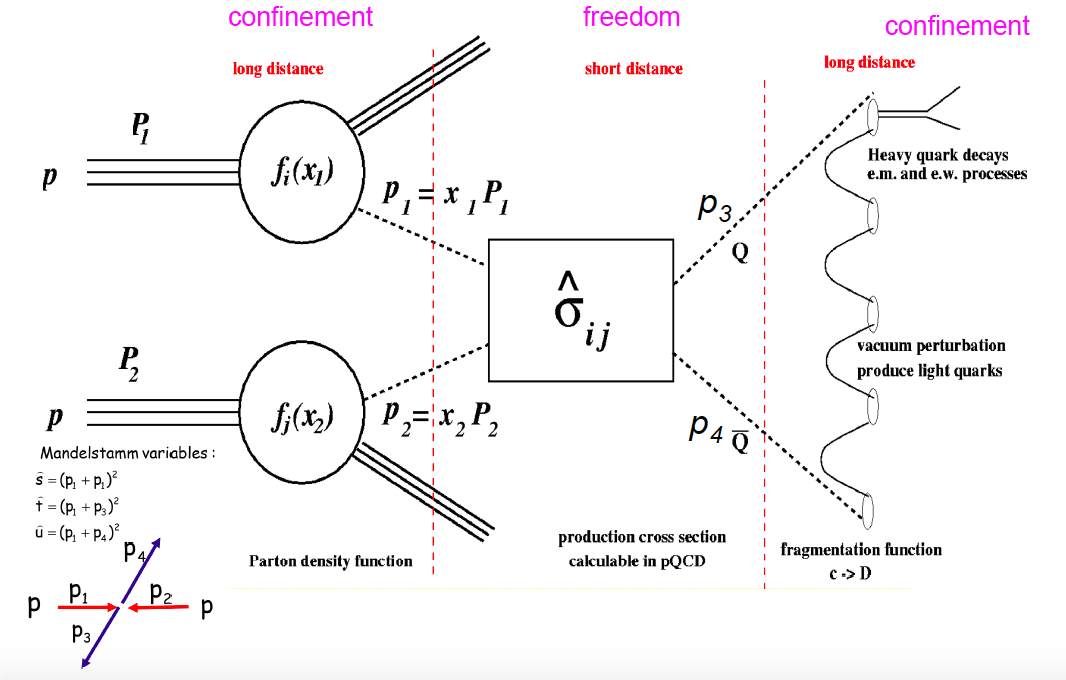
\includegraphics[width=0.75\textwidth]{Figures/Chapter1/QCDFactorizationTheorem.png}
\caption{The QCD factorization theorem applied to a pp collision event involving in soft and hard processes are shown above.}
\label{QCDFacTheo}
\end{center}
\end{figure} 

The hard processes are encoded in the factor of partonic cross sections while the soft processes are measured in experiments. Physicists developed parton distribution function to describe initial kinematic of partons inside hadrons and fragmentation function to describe the parton hadronization process. Both parton distribution function and fragmentation function are measured in experiments.


Physicists apply QCD factorization theorem to perform pQCD calculation of hard scattering processes and use the measurement from the  to understand the hadron spectroscopy in electron-positron, electron-proton, and proton-proton collisions.

\subsection{Color Confinement}

Another feature of QCD as a non-abelian gauge theory is color confinement. The strong force carrier gluon itself is also color charged. Color charged partons, namely quarks and gluons, are never detected in isolation. In experiments, only color neutral hadrons are detected. Currently, the analytic explanation of color confinement is still not yet rigorously proven. The theoretical explanation of color confinement in QCD remains one of the unsolved problem in physics. 

\subsection{Hadronization}

The formation process hadrons from partons is called haronization. Because in experiments we only measure final state hadrons, in order to study the interactions and dynamics of quarks and gluons during partonic stage from hadron spectra, we also need to understand hadronization mechanisms. However, hadronization is in general non-perturbative and cannot yet be described by first principle QCD calculations. Therefore, physics make phenomenological models such as the Statistical Hadronization Model \cite{SHM}, Lund String Model \cite{LSM}, Quark Coalescence Model \cite{QCM} to study hadronization. Figure  \ref{HadMech} shows the schematics of hadronization of a beauty quark via fragmentation and coalescence process.

\begin{figure}[hbtp]
\begin{center}
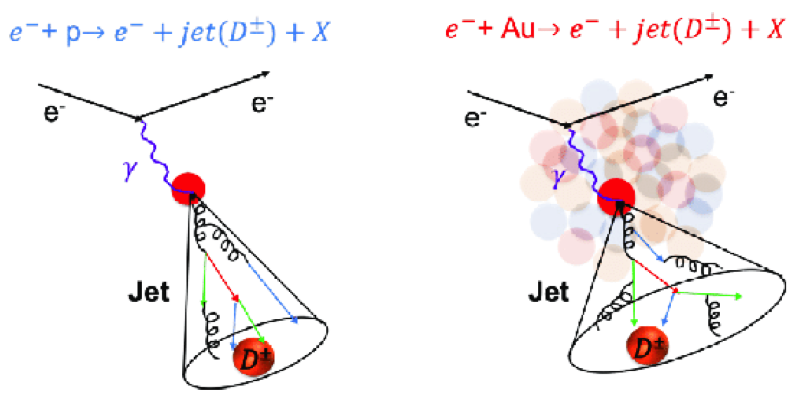
\includegraphics[width=0.48\textwidth]{Figures/Chapter1/FragCartoon.png}
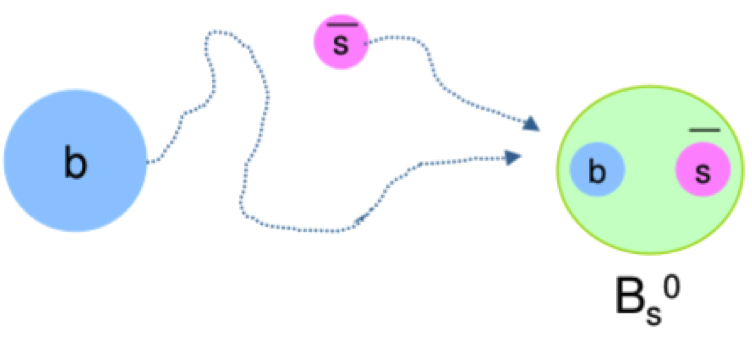
\includegraphics[width=0.48\textwidth]{Figures/Chapter1/CoalCartoon.png}
\caption{The fragmentation process of charms quarks hadronize into $D^\pm$ (left) and the coalescence process of beauty quark with a strange quark nearby to form a $B^0_s$ are shown above.}
\label{HadMech}
\end{center}
\end{figure} 

\section{QCD In Extreme Conditions}

Historically, many efforts to understand QCD in extreme conditions have been made \cite{QCDExtreme}. There are mainly two directions: temperature and parton density. Figure~\ref{QCDConds} shows the different studies of QCD in different conditions \cite{QCDDiffConds}:


\begin{figure}[hbtp]
\begin{center}
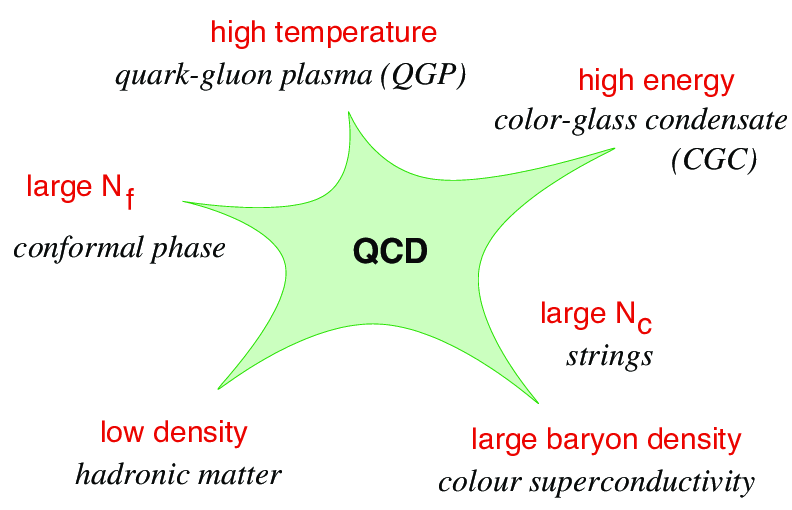
\includegraphics[width=0.70\textwidth]{Figures/Chapter1/ManyBodyQCD.png}
\caption{Many-body dynamics of QCD in different physics limits is shown above.}
\label{QCDConds}
\end{center}
\end{figure} 

\subsection{QCD at Finite Temperature}

In QCD, under extremely high energy density, the degree of freedom of the system increases via particle production. Many-body dynamics become relevant. In the limit of large number of quarks and gluons, after a sufficiently long period of time, the system reach thermal equilibrium via strong interaction \cite{MLBThermal,ADSCFTThermal,QCDThermal}. Therefore, a description based on thermodynamics can be formulated to study such systems \cite{QCDThemDyn}. We call this thermalized and strongly interacting many-body system of quarks and gluons to be QCD matter.

Therefore, an additional variable temperature ($\mathbf{T}$) can be introduced to study such QCD systems. There are some interesting QCD phenomenologies involving temperature as listed in the following subsections.

%\vspace{1.0cm}

\subsection{Melting of QCD Vacuum}

The QCD vacuum is filled with various condensates of quarks-antiquark pair and gluon fields \cite{QCDVacuum}. In the QCD vacuum, the three flavor of light quarks: $u$, $d$, $s$ form a flavor symmetry group of $SU(3)_f$. However, for quark-quark pair, the $SU(3)_f \times SU(3)_f$ chiral symmetry is spontaneously broken. For example, in the vacuum, a quark-antiquark pair field has a non-vanishing expectation value of $\bra{0} \bar \psi (x)  \psi(x) \ket{0} \simeq$ (250 MeV)$^3$ \cite{}. Therefore, in the physical QCD vacuum, all color field are confined in hadrons. In 1974 T.D. Lee formulated the idea that the non-perturbative vacuum condensates could be ``melted down ... by distributing high energy or high nucleon density over a relatively large volume'' \cite{StockR,QCDVacMelt}. As the energy density in space increases, the color field start to permeate all space. This is effective melting the QCD Vacuum as the temperature of the system increases. Therefore, the temperature of the system will affect the QCD vacuum structure. 

%\vspace{1.0cm}

\subsection{Chiral Symmetry Restoration}

At a finite critical temperature $T_c > 0$, the quark-antiquark pair field will have a vanishing expectation value. In this scenario, massive quarks behave as if massless \cite{ChiralTemperature}. Thus, the chiral symmetry of quarks is restored \cite{ChiralRestore}. Therefore, under a strong magnetic field, due to the restored chiral symmetry, the quarks generate anomalous chiral current $j^{\mu}_{5}$ described by $U(1)_A$ chiral anomaly, calculated by the famous ``Triangle Feynman diagram'' in Figure~\ref{ChiralFeynman} shown below:



\begin{figure}[hbtp]
\begin{center}
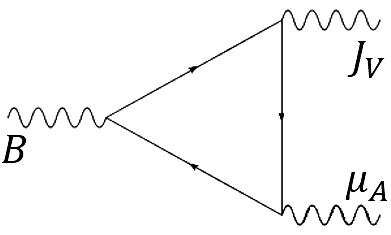
\includegraphics[width=0.45\textwidth]{Figures/Chapter1/ChiralTriangle.png}
\caption{The Feynman diagram of a triangular quark loop under external magnetic field $B$ describe the generation of chiral magnetic current via chiral anomaly is shown above.}
\label{ChiralFeynman}
\end{center}
\end{figure} 


The anomalous chiral current $j^{\mu 5}$ is given by \cite{ChiralPaper}

\begin{equation}
\partial_\mu j^{\mu}_{5} =  - \frac{N_{f}g^2}{16 \pi^2} G^{\mu\nu}_a \widetilde{G^a_{\mu\nu}}
\end{equation}

Here $G^{\mu\nu}_a$ is defined as

\begin{equation}
\widetilde{G^a_{\mu\nu}} = \frac{1}{2} \epsilon_{\mu\nu\lambda\sigma}G^{\lambda\sigma a}
\end{equation}


According to the continuity equation of chiral current

\begin{equation}
\frac{\partial \rho_5}{\partial t} + \nabla \vec{j_5} = 0 
\end{equation}

By definition, the chiral current $\rho_5$ is the difference of the right-handed charge $\rho_L$ and left-handed charge $\rho_R$.


In terms of number of particles $N_5 = \frac{Q_5}{e} = \int  {\rho_5}{e} d^3x$, integrating both sides by the spatial volume and divide by the volume, we have



\begin{equation}
\frac{d N_5}{dt} =  \int d^3x \nabla \vec{j_5} = \int  - \frac{N_{f}g^2}{16e \pi^2} G^{\mu\nu}_a \widetilde{G^a_{\mu\nu}} d^3x 
\end{equation}


The chiral chemical potential $\mu_5$ is proportional to the number of particle $N_5$: $j_5 \propto N_5$ This non-vanishing anomalous chiral current implies non-zero chiral magnetic dipole moment density $\mu_5 \ne 0$. Finally, under an external magnetic field, the induced electric current $j^\mu_V$ is given by  


\begin{equation}
\vec J_V = \frac{N_c e}{2\pi^2} \mu_A \vec B \ne 0
\end{equation}

In experiments, we should expect to see the separation of left-handed and right-handed quarks $Q_V$ due to this electric current $\vec J_V$ where charge imbalance between the positive and negative direction along the magnetic field \cite{CMESignature} as $\Delta Q = \int_0^\tau \vec J_V \cdot \vec A dt \ne 0$. We call this chirality imbalance effect due to the restored chiral symmetry of quarks at finite temperature as \textbf{Chiral Magnetic Effect} \cite{RestoreCME}. Figure~\ref{ChiralScheme} illustrates the schematics of Chiral Magnetic Effect in Heavy-Ion Collisions \cite{CMEFigPaper}

\begin{figure}[hbtp]
\begin{center}
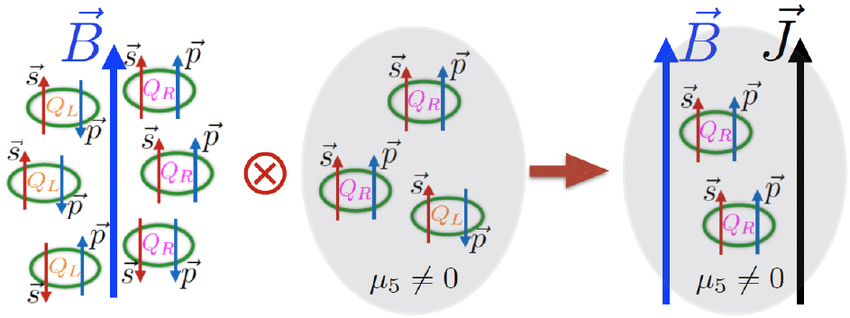
\includegraphics[width=0.70\textwidth]{Figures/Chapter1/ChiralScheme.png}
\caption{The schematics of charge separation due chirality imbalance of quarks under a strong magnetic field in heavy-ion collisions, know as Chiral Magnetic Effect, is shown above.}
\label{ChiralScheme}
\end{center}
\end{figure} 


Currently, physicists are actively looking for evidences of Chiral Magnetic Effect in experiments but have not yet reported any conclusive results so far \cite{CMEExpResult}. 

%\vspace{1.0cm}

\subsection{Temperature Dependence of QCD Static Potential}. 

If we consider two quarks in the limit of finite mass and are essentially at rest in the lab frame, we can define a QCD static potential between these two quarks due to the strong interaction. In vacuum, such a potential is called ``Cornell Potential'' \cite{Cornell}. The potential as a function of the distance between two quarks is shown as follows:

\begin{equation}
V(r) = -\frac{\alpha_{eff}}{r} + \sigma r
\end{equation}

Here, $\alpha_{eff}$ is the effective strong coupling coupling between the two quarks and $\sigma \simeq 0.184$ GeV/c is the string coupling constant \cite{CornellEquation}. 

Now if we consider at finite temperature T with a thermalized system  between the two quarks, the QCD static potential becomes: 

\begin{equation}
V(r) = -\frac{\alpha_{eff}}{r} e^{-m_D r} + \frac{\sigma}{m_D} (1 - e^{-m_D r})
\end{equation}

Here, $m_D \sim g_s T$ is the Debye mass due to Debye color screening effect \cite{CSEff}, which essentially modifies the gluon propagator by inserting a finite mass term: $-i \frac{g^{\mu\nu}}{q^2} \rightarrow -i \frac{g^{\mu\nu}}{q^2 - m_D^2}$. In fact, Equation (2) reduces to the Cornell potential when T = 0. The QCD static potential is shown below in Figure~\ref{QCDPotential}


Many interesting physics implications can be deduced from QCD at finite temperature.


\subsection{Hadron Mass Spectrum and Hagedorn Temperature}

In 1965, Hagedorn proposed a statistical thermodynamically bootstrap model, giving the temperature dependence of hadron spectra \cite{Hagedorn}. According to the principle of asymptotic bootstrap, in the limit of high mass resonance $m \rightarrow \infty$ the mass spectrum of hadrons $\rho(m)$ grows exponentially 

\begin{equation}
\rho (m) \propto m^{-\frac{5}{2}} e^{\frac{m}{T_0}}
\end{equation}

Here, $\rho(m)$ dm stands for the number of excited hadron with mass between $m$ and $m+dm$. $T_0 \simeq 158$ MeV is the temperature parameter extract from experiments. As $T \rightarrow T_0^-$, $\rho(m) \rightarrow \infty$. The mass spectrum of hadrons diverges. Therefore, it stands for the highest possible temperature achievable for the strong interaction between hadrons. Hence, $T_0$ is also called the ``Hagedorn Temperature''. For $ T > T_0$, the description of color-neutral hadrons mass spectrum will break down, indicating a new type of matter with deconfined degree of freedom in the interaction \cite{HagedornDeconfine}.

\subsection{Color Deconfinement}

As mentioned in the sections above, we see that, at finite temperature, the QCD static potential is screened and color degree of freedom become relevant in the system. As the temperature of the system increase, the quarks and gluon inside color-neutral hadrons will have more available space to move around and start to deconfine \cite{DeconfineTemp}. At some critical temperature $T_c$, quarks and gluons will form a new type color deconfined QCD matter, which is called Quark-Gluon Plasma (QGP). The typical temperature of QGP is in the order of a few hundred MeV or about $10^{12}$ K, which is about a million times hotter than the core of the Sun.

\subsection{QCD at High Parton Density}

In the other direction, while keeping zero temperature, by increasing density of the color fields of the system, another form of QCD matter will also emerge \cite{CondensedQCD}.. Due to confinement, a single quark or gluon cannot exit in vacuum. Therefore, the simplest form of QCD system will be a meson, which consist of one quark and one antiquark. The next more complex system will be baryon, for instances, nucleons, which consistent of three quarks. We can then use nucleons to form atomic nuclei and even neutron stars. As the number of nucleons in the system increases, the nucleon density also increases, which increase the color field density. Below, we will discuss the consequence of increasing color field density by increasing the color field lines and decreasing the volume of the system. In general, we can study QCD at High Parton Density by probing small$-x$ physics \cite{SmallX}  


\subsection{Color Glass Condensate}

One way to increase the color field density is by decreasing its volume. The radius of a hadron will shrink due to the Lorentz contraction effect as it moves with respect to the spectator. However, since the number of color charges inside the does not change, the color field density will increase. At very high energy, the hadrons will turn into ``gluon walls'' \cite{GluonWalls} and form a dense color field of matter \cite{DenseColorField} named Color Glass Condensate is formed \cite{CGCPaper}.

\subsection{Nuclear Shadowing}

At high energy, or equivalently, small $x$, according to the QCD evolution equation, the gluons inside the nucleon of the nuclei will ``create shadows" on each other \cite{IntroShadow}, The high density effects results in the modification of the nuclear structure function and the gluon nucleon parton distribution \cite{DenseQCD}. Therefore, in high energy hadron-nucleus collision, we expect to see the decrease of cross section per participant nucleons at small-$x$ region compared other $x$ region \cite{ExShadow}. We call this effect as ``nuclear shadowing (of gluons)'' \cite{NuclearShadowing}. 
\section{QCD Matter}

\subsection{QCD Phase Diagram}

Similar to form everyday matters such as metal, water, wood, glass, and plastic, which are formed by electromagnetic interaction and could all be described macroscopically by equations of states that are parameterized by thermodynamic variables. Figure~\ref{QEDPhaseDiagram} shows the phase diagram of water ($\mathrm{H_2O}$) at different temperature and pressure:

\begin{figure}[hbtp]
\begin{center}
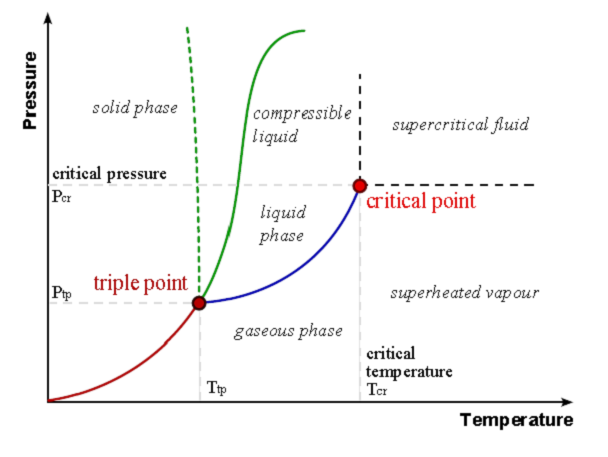
\includegraphics[width=0.45\textwidth]{Figures/Chapter1/WaterPhaseDiagram.png}
\caption{The P-T diagram of water in gas, liquid, solid phases is shown above.}
\label{QEDPhaseDiagram}
\end{center}
\end{figure} 


Similarly, QCD matter is the matter formed by numerous quarks and gluons via the strong interaction and can also be describe by equations of states. Like our everyday matter which has gas, liquid, and solid phases at different pressure and temperature, QCD matter also has different phases at different temperature and baryon chemical potential. and can be describe by QCD phase diagrams. Figure~\ref{QCDPhaseDiagram} shows the QCD phase diagram at different temperature and baryon chemical potential:

\begin{figure}[hbtp]
\begin{center}
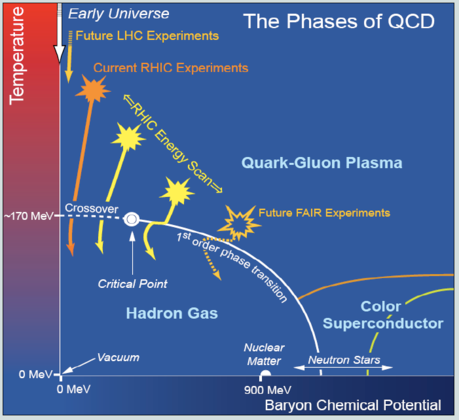
\includegraphics[width=0.45\textwidth]{Figures/Chapter1/QCDPhaseDiagram.png}
\caption{The theoretical QCD phase diagram of different QCD matter, including hadron resonance gas, quark-gluon plasma, neutron star, and color superconductor, as function of temperature and baryon chemical potential is shown above. The solid line indicates the conjecture of first order phase transition between quark-gluon plasma and hadron gas while the dash line is a smooth crossover.}
\label{QCDPhaseDiagram}
\end{center}
\end{figure} 

\subsection{Hadron Resonance Gas}

One of the most familiar type of QCD matter is hadron resonance gas, which lies at the left bottom corner of the QCD phase diagram. Hadron resonance gas is a system of color neutral hadrons at relative low temperature. The interaction between hadrons are the Van der Waas like strong nuclear force as the residue of the color force via exchange of mesons. The strong nuclear force between two nucleons shown below Figure \ref{NuclearForce}. 

\begin{figure}[hbtp]
\begin{center}
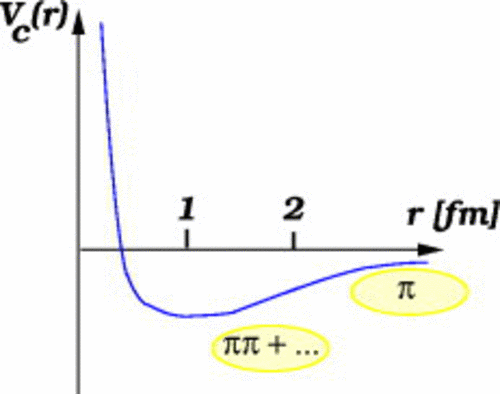
\includegraphics[width=0.45\textwidth]{Figures/Chapter1/NuclearForce.png}
\caption{The schematic plot of potential energy between two nucleon via pion exchange as a function of distance is shown above \cite{StrongNuclear}. This potential with a well minimizing near 100 MeV allow nucleons to bind together and form atomic nuclei and nuclear matter.}
\label{NuclearForce}
\end{center}
\end{figure} 

The equation of state of non-interacting hadron resonance gas could be described by grand canonical ensemble of bosons (mesons) and fermions (baryons) \cite{StatMechHadron}. We should note that pions dominates the hadron gas at low temperature. The realistic equation of state of hadron resonance gas should also consider the interaction. An example of the equation of state of hadron resonance gas consider the Van der Waas interaction comparing with lattice QCD simulation is given in Figure \ref{EOSHadronLattice} below \cite{EOSHadron}:

\begin{figure}[hbtp]
\begin{center}
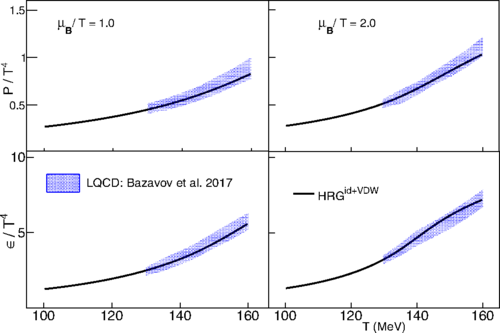
\includegraphics[width=0.45\textwidth]{Figures/Chapter1/EOSHadronGas.png}
\caption{The pressure and energy density from lattice simulation compared with ideal hadron resonance gas and Van der Waas interaction at different $\frac{\mu_B}{T}$ are shown above.}
\label{EOSHadronLattice}
\end{center}
\end{figure} 



Nuclear matter is considered as part of the hadron resonance gas in the QCD phase diagram. Examples of typical hadron gas will be atomic nuclei at a famous nuclear matter saturation density $n_S$ = 0.16 $fm^{-3}$ (baryon density $n_B = 3 n_S$) and nuclear matter like neutron star at large baryon density. 

\subsection{Quark-Gluon Plasma}

At very high temperature, quarks and gluons inside the color neutral hadron resonance gas will deconfine and form a new type of matter called quark-gluon plasma (QGP). In cosmology, it is believed that QGP exists in the early universe just several microseconds after the Big Bang during the quark epoch after electroweak phase transition and before nucleosynthesis \cite{QGPCosmology}. 

The temperature of QGP is in order of hundreds of MeV, which is a about a million times hotter than the core of the Sun. Moreover, according to extensive experimental and theoretical studies, QGP demonstrates strongly coupled ideal liquid behavior, which directly contracts to the prediction from asymptotic freedom which predict such matter should behavior like a gas of weakly interacting quarks and gluons. Therefore, the inner workings and proper degrees of freedom of QGP must be somewhere in between weakly coupled quarks and gluons and color neutral hadrons because it still demonstrate significant color freedom due to deconfinement. However, the microscopic structure of QGP is still unknown. Currently, both experimental and theoretical efforts have been conducted to actively investigate the internal structure of QGP.

Based on its ideal liquid feature, QGP could be described by relativistic viscous hydrodynamics. In fact, the quantum limit predicted by the Anti-de-Sitter Space Conform Field Theory (AdS/CFT). It is about a factor of larger than water.

The accurate equation of state of QGP is currently unknown. According to MIT Bag Model, the energy density $\epsilon$ and pressure $p$ of a plasma of free quarks and gluons as a function of temperature $T$ is as follows \cite{MITBag}:

\begin{equation}
\epsilon = \frac{37 \pi^2}{30} T^4 + \mathcal{B}
\end{equation}

\begin{equation}
p = \frac{37 \pi^2}{90} T^4 - \mathcal{B}
\end{equation}

Here, $\mathcal{B}$ is the Bag Constant, which can be understood as the pressure of the vacuum on the quarks and gluons to make them form hadrons with finite size.

If we represent $p$ in terms of $\epsilon$, we get

\begin{equation}
p = \frac{1}{3} (\epsilon - 4B)
\end{equation}

\subsection{Color Superconductor}

Under extremely high net baryon density, there is another hypothetical state of QCD matter named Color Superconductor where the color charges can move freely \cite{ColorSuperconductor}. Similar to the Cooper Pair formation mechanism of electrons in metals, quarks, as fermions, pair up and bosonized into diquark, and undergo Bose-Einstein condensation \cite{ColorSuperconductor}. The diquark condensate, carrying color charges, can move without resistance and thus demonstrate color superconductivity. It is believed that the color superconductor exists in the core of neutron stars where the net baryon chemical potential is high \cite{CSCOccurrence}. However, so far no color superconductor has been discovered in laboratory or astrophysical observations. 

\subsection{Phase Transition}

As we increase the temperature, hadron resonance gas will undergo a phase transition into QGP. The chiral symmetry is restored from the phase transition of hadron resonance gas to QGP. However, the order of the phase transition from resonance hadron to QGP is still unknown. According to lattice QCD calculations, near zero baryon chemical potential ($\mu_B = 0$), the phase transition is a smooth cross over. However, at finite baryon chemical, it is believe that the phase is a first order phase transition according to different model calculations \cite{QCDFirstOrder}. The hint of first order phase transition can be found in the softening equation of state in the cross over region \cite{EOSPhase}. However, currently, the order of phase transition from hadron resonance gas to QGP at high baryon chemical potential is still an open question. %However, there is no direct physical observable to determine the order of the phase transition in experiments \cite{Observables}.

\subsection{Critical Point}

If the theoretical predictions are correct, according to thermodynamics, there must be a critical point between the first order phase transition and the smooth crossover. Theoretical calculations predict that the critical point is $\mu_B = $ 350 -- 700 and $T_{c}$ $\approx$ 160 MeV \cite{CriticalPointTH}. Experimentally, the scale of the critical temperature may occur at $T_{c}$ $\approx$ 175 MeV from high moment analyses \cite{CriticalPointEX}. The research on critical point, a landmark in the QCD phase diagram, and the phase transition between QGP and hadron resonance gas are very important topics for physicists to understand the nature of QCD matters. The STAR Collaboration has carried out a Beam Energy Scan, both Phase I and II, at RHIC and plan to extend it to higher baryon chemical ponetial and lower temperature in the future Fixed Target Mode to search the critical point in the QCD phase diagram. However, so far efforts to search the precise locations of the critical point is still ongoing. The results are still inconclusive \cite{STARBES}. 

\section{High Energy Nuclear Physics}

\subsection{Laboratories}

In laboratories, physicist collider heavy nuclei at high energy to study QCD under extremely hot and dense condition.

\subsection{Heavy-Ion Accelerators}

\subsection{Heavy-ion Physics Detectors}

\subsection{Stages of Heavy-Ion Collisions}

\subsection{Coordinates}

\subsection{Glauber Model}

\section{The Quest for the Quark-Gluon Plasma}

\subsection{Signatures}

\subsection{Discovery}

\subsection{Properties}

%Nuclear Physics is a study of the interaction of nucleons and structure of atomic nuclei. 
\subsection{Microscopic Structure}

\subsection{Open Questions}


\section{Hard Probes}

\subsection{Jets}

\subsection{Electroweak Probes}

\subsection{Heavy Quarks}

\section{Open Heavy Flavor Physics}

\subsection{Heavy Quark Diffusion}

\subsection{Heavy Quark Energy Loss}

\subsection{Heavy Quark Hadronization}

\subsection{Experimental Observables}




